\begin{center}
        	\begin{tikzpicture}
	\node[anchor=south west,inner sep=0] (image) at (0,0) {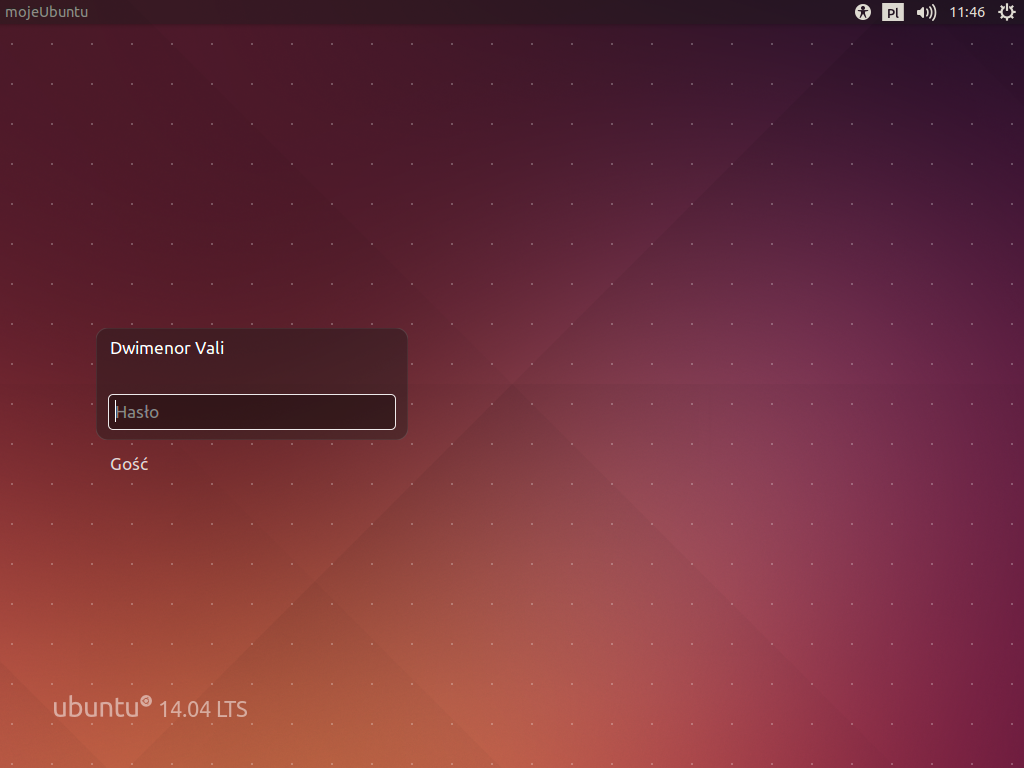
\includegraphics[width=\linewidth]{images/greater.png}};
	\begin{scope}[x={(image.south east)},y={(image.north west)}]
		\draw[ubuntu_orange,line width=3pt,rounded corners] (0.1,0.52) rectangle (0.23,0.57);
		\draw[ubuntu_orange,line width=3pt,fill=white,fill opacity=0.75] (0.45,0.55) circle [radius=0.30cm]
			node[text=black]{\Large \textbf 1};
		\draw[ubuntu_orange,dashed,line width=3pt] (0.43,0.55) -- (0.23,0.55);
		
		\draw[ubuntu_orange,line width=3pt,rounded corners] (0.1,0.44) rectangle (0.39,0.49);
		\draw[ubuntu_orange,line width=3pt,fill=white,fill opacity=0.75] (0.45,0.47) circle [radius=0.30cm]
			node[text=black]{\Large \textbf 2};
		\draw[ubuntu_orange,dashed,line width=3pt] (0.43,0.47) -- (0.39,0.47);
		
		\draw[ubuntu_orange,line width=3pt,rounded corners] (0.1,0.38) rectangle (0.23,0.42);
		\draw[ubuntu_orange,line width=3pt,fill=white,fill opacity=0.75] (0.45,0.40) circle [radius=0.30cm]
			node[text=black]{\Large \textbf 3};
		\draw[ubuntu_orange,dashed,line width=3pt] (0.43,0.40) -- (0.23,0.40);
		
		\draw[ubuntu_orange,line width=3pt,rounded corners] (0.00,0.96) rectangle (0.10,1.00);
		\draw[ubuntu_orange,line width=3pt,fill=white,fill opacity=0.75] (0.05,0.85) circle [radius=0.30cm]
			node[text=black]{\Large \textbf 4};
		\draw[ubuntu_orange,dashed,line width=3pt] (0.05,0.87) -- (0.05,0.96);
		
		\draw[ubuntu_orange,line width=3pt,rounded corners] (0.82,0.96) rectangle (1.00,1.00);
		\draw[ubuntu_orange,line width=3pt,fill=white,fill opacity=0.75] (0.90,0.85) circle [radius=0.30cm]
			node[text=black]{\Large \textbf 5};
		\draw[ubuntu_orange,dashed,line width=3pt] (0.90,0.87) -- (0.90,0.96);
    \end{scope}
\end{tikzpicture}
\end{center}

W czasie ładowania systemu operacyjnego będzie widoczne logo Ubuntu ze stopniowo wypełniającymi się kwadratami. Po wciśnięciu dowolnego klawisza logo zostanie zastąpione szczegółowym opisem tego, co jest aktualnie wykonywane.
Kiedy proces uruchamiania systemu dobiegnie końca, zobaczysz ekran logowania Ubuntu (jeżeli w czasie instalacji wybrałeś \textcolor{ubuntu_orange}{Automatyczne logowanie}, to ten krok zostanie pominięty i od razu włączy się Pulpit).
\begin{enumerate}[label=\protect\circled{\arabic*}]
\item Lista użytkowników systemu. Jeżeli w systemie jest więcej niż jeden użytkownik, to z tej listy będzie można wybrać kto ma zostać zalogowany.
\item W to pole wpisz hasło aktualnie wybranego użytkownika.
\item Konto ,,Gość'' umożliwia zalogowanie się do systemu bez podawania hasła. Wszystkie zmiany wprowadzone przez gościa (np. utworzone pliki) zostaną utracone po zakończeniu sesji.
\item Nazwa systemu wybrana podczas instalacji.
\item Przyciski sterujące:
\begin{description}
\item[
\includegraphics{images/ikony_dostempnosc.png}] \textcolor{ubuntu_orange}{Dostępność} --- uruchomienie lupy, czytnika ekranowego lub klawiatury ekranowej;
\item[
\includegraphics{images/ikony_jezyk.png}] \textcolor{ubuntu_orange}{Język} --- pozwala zmienić układ klawiatury i metodę wprowadzania tekstu;
\item[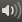
\includegraphics{images/ikony_dzwiek.png}] \textcolor{ubuntu_orange}{Ustawienia głośności i dźwięku};
\item[\textbf{11:46}] \textcolor{ubuntu_orange}{Zegar i kalendarz};
\item[
\includegraphics{images/ikony_zasilanie.png}] \textcolor{ubuntu_orange}{Zasilanie} --- wyłączenie lub ponowne uruchomienie komputera.
\end{description}
\end{enumerate}
